\documentclass{article}
\usepackage{xeCJK} % 中文支持
\usepackage{fontspec} % 字体设置
\setCJKmainfont{SimSun} % 设置中文主字体
\setmainfont{Times New Roman} % 设置英文主字体

\usepackage{polyglossia} % 语言支持
\setdefaultlanguage{english}
\setotherlanguages{japanese, chinese}

\usepackage{graphicx} % 图片
\usepackage{caption}  % 用于美化标题

% % 脚注
% \usepackage{mpfnmark}
% \usepackage{fancyhdr}
% \usepackage[savemap]{footnote}

% \pagestyle{fancy}
% \fancyhf{} % 清除默认的页眉和页脚

% % 在页脚中添加脚注内容
% \fancyfoot[C]{%
%   \vspace{1em}%
%   \footnotesize%
%   \rule{\textwidth}{0.4pt}\\ % 分隔线
%   \Footnotetexts%
% }

\linespread{1.25} % 行距

% 日文支持
\newfontfamily\japanesefont{MS Mincho}
\newcommand{\jp}[1]{{\japanesefont #1}}

\begin{document}

\tableofcontents % 生成目录
\newpage

\section{入境之前}
使用iPhone设备在钱包(Wallet)中添加Suica(即俗称的西瓜卡), 可以通过Apple Pay从国内银行卡直接充值,准备一张NFC西瓜卡极其重要。(安卓系统操作方式不知道捏)\par
现在入境申报已经电子化,在入境之前事先准备QR码可以极大加速入境流程。另外,最好不要带100万以上的日元现金在身上,需要额外申报,很麻烦。\par
\section{行:行こうよ!}
\subsection{机场}
东京一共有两个机场:羽田(はねだ,haneda)机场和成田(なりだ,nanida)机场,地理位置都相对远离市区。因为汉字和读音接近的缘故,两个机场很容易弄混,出发前请务必确认清楚(不要问我是怎么知道的)。\par
由于羽田是新机场,所以一般是相对高价的航班,且羽田机场结构相对紧凑,例如单轨电车站与到达大厅直接相连,而在成田需要走的路就比较多了,但是成田机场航站楼之间的通道是宝可梦题材的装修(成田上大分)。\par
两个机场都有电车直通山手线的车站(山手线的战略意义见后文),其中成田机场的电车是京成電鉄运营的天空快线(スカイライナー,sukairainaa),直达日暮里(にっぽり,nippori)站:
\begin{figure}[h!]
    \centering
    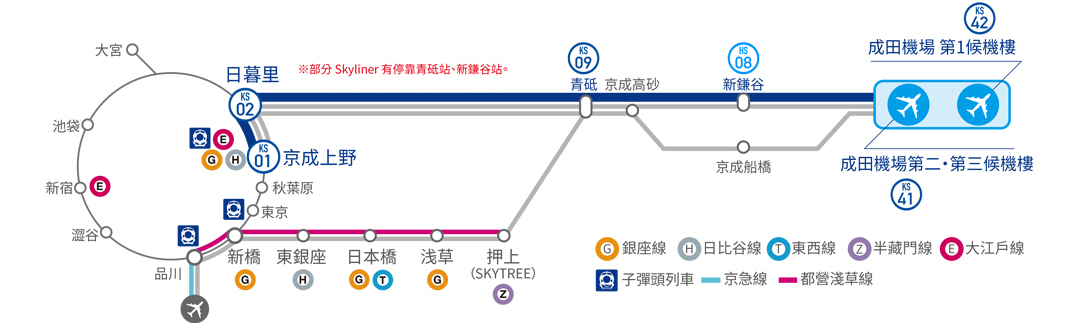
\includegraphics[width=0.9\textwidth]{./fig/routemap_skyliner.jpg} % 替换为您的图片文件
    \caption{天空快线(スカイライナー)线路图\protect\footnotemark}
\end{figure}
\footnotetext{来源:https://www.keisei.co.jp/keisei/tetudou/skyliner/jp/index.php}

羽田机场则是单轨电车(モノレール)连接的则是浜松町(はままつちょう,hamamatucyou)站:
\begin{figure}[h!]
    \centering
    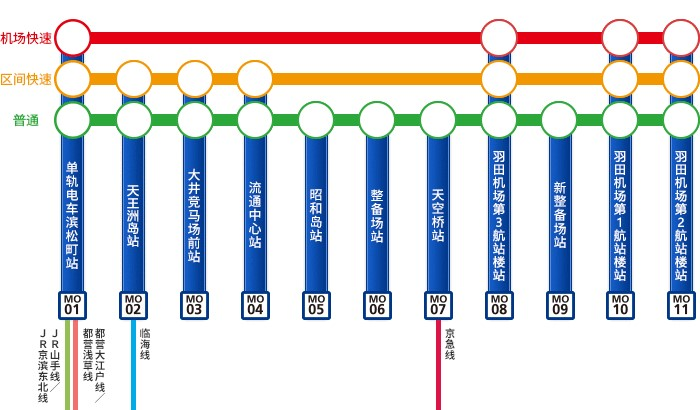
\includegraphics[width=0.6\textwidth]{./fig/routemap_monorail.jpg} % 替换为您的图片文件
    \caption{单轨电车(モノレール)线路图\protect\footnotemark}
\end{figure}
\footnotetext{来源:https://www.tokyo-monorail.co.jp/sc/guidance/index.html}

P.S.\par
全日空(ANA)在羽田有专门的check in区域。\par
两个机场都有大巴车通往包括富士山在内的各种重要地方,但是我没坐过,pass。

\subsection{电车/地铁}


\section{吃:食べましょう!}

\section{景点}


\section*{测试文本 テスト}
这是一段中文文本。\par
\jp{これは日本語の文章です}あいうえお。\par
This is a paragraph in English.


\end{document}